\documentclass[12pt, a4paper]{article}
\usepackage[francais]{babel}
\usepackage{pgfplots}
\usepackage{caption}
\usepackage{graphicx}
\usepackage[T1]{fontenc}
\usepackage{listings}
\usepackage{geometry}
\usepackage{minted}
\usepackage{array,multirow,makecell}
\usepackage[colorlinks=true,linkcolor=black,anchorcolor=black,citecolor=black,filecolor=black,menucolor=black,runcolor=black,urlcolor=black]{hyperref}
\setcellgapes{1pt}
\makegapedcells
\usepackage{fancyhdr}
\pagestyle{fancy}
\lhead{}
\rhead{}
\chead{}
\rfoot{\thepage}
\lfoot{Martin Baumgaertner}
\cfoot{}
\renewcommand{\footrulewidth}{0.4pt}
\renewcommand{\headrulewidth}{0.4pt}
\renewcommand{\listingscaption}{Code}
\renewcommand{\listoflistingscaption}{Table des codes}
% \usepackage{mathpazo} --> Police à utiliser lors de rapports plus sérieux

\begin{document}
\begin{titlepage}
	\newcommand{\HRule}{\rule{\linewidth}{0.5mm}} 
	\center 
	\textsc{\LARGE iut de colmar}\\[1.5cm] 
	\textsc{\Large R303}\\[0.5cm] 
	\textsc{\large Année 2022-23}\\[0.5cm]
	\HRule\\[0.75cm]
	{\huge\bfseries Services réseaux avancés}\\[0.4cm]
	\HRule\\[1.5cm]
	\textsc{\large martin baumgaertner}\\[0.5cm] 

	\vfill\vfill\vfill
	{\large\today} 
	\vfill
\end{titlepage}
\newpage
\tableofcontents
\listoffigures
\newpage
\section{CM 1 - 6 septembre 2022}
\subsection{Rappels}
TCP : permet d'avoir une communication fiable de bout en bout, on a une session 
qui permet de faire du recouvrement, s'il y a un paquet perdu on le retransmet, pour ça on 
utilise un numéro de séquence, et on a un mécanisme d'aquittement qui nous dit quel
octet est arrivé et quel octet est perdu. \\

UDP : est utilisé lorsque l'accusé de réception des données n'a aucune signification, 
est un bon protocole pour les données circulant dans une seule direction,
est simple et adapté aux communications basées sur des requêtes,
n'est pas orienté connexion,
ne fournit pas de mécanisme de contrôle de congestion.\\

\begin{figure}[H]
    \centering
    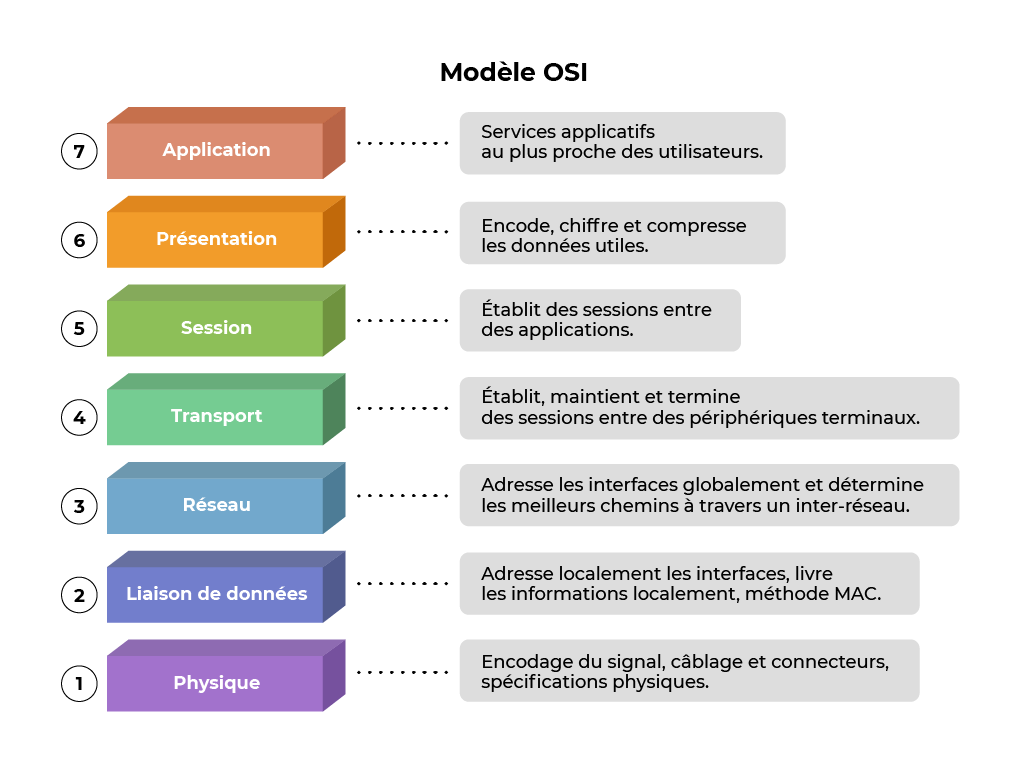
\includegraphics[width=0.9\textwidth]{img/osi.png}
    \caption{Le modèle OSI}
    \label{fig:osi}
\end{figure}
\newpage
\subsection{Les DNS}
Le Domain Name System (DNS) est une base de données distribuée organisée de manière
hiérarchique, un protocole applicatif qui permet à un hôte de l'intérrroger. Le
port utilisé par défaut pour DNS est le port 53. L'objectif de ce sytème est
d'identifier les hôtes grâce à un nom. \\
Le système DNS est souvent utilisé en amont des protocoles applicatifs comme 
HTTP ou les mails.\\

\begin{figure}[H]
\centering
\begin{tikzpicture}
    \begin{axis}[	grid= major ,
            width=0.7\textwidth ,
            xlabel = {Année} ,
            ylabel = {Nombre (en milliard)} ,
            xmin = 1991, xmax = 2022,
            ymin = 0, ymax = 7 000 000 000,
            legend entries={Nombre site web, Nombre d'internautes},
            legend style={at={(0,1)},anchor=north west}]
        \addplot coordinates {(1991,1) (2001,29 000 000) (2011,346 000 000) (2022,2 000 000 000) }; % Tracé point à point
        \addplot coordinates {(2000,414 000 000) (2005,1 000 000 000) (2011,2 000 000 000) (2022,5 000 000 000) }; % Tracé point à point
       
    \end{axis}
\end{tikzpicture}
\caption{Nombre de site web et d'internautes en fonction des années}
\end{figure}
    
    \subsubsection{Fonctionnement du DNS}
    Le DNS gère la distribution du trafic : distribue les informations
    reçus sur le site voulu sur les 2 adresses IP du site.
    Un serveur racine du DNS est un serveur DNS qui répond aux requêtes qui concernent les noms de
    domaines du premier niveau et qui les redirige vers le serveur DNS de premier niveau concerné.
    Bien qu'il puisse exister d'autres hiérarchies de systèmes de noms de domaine (DNS) avec des serveurs
    racine alternantifs, "serveur racine du DNS" est généralement utilisé pour 
    désigner l'un des serveurs racine du DNS d'internet gégé sous l'autorité de L'ICANN.
\newpage 
\subsection{Créer des raccourcis (alias)}
Un alias est un raccourcis dans l'URL d'un site web, on peut donc passer de \\www.iutc078.uha.fr.iut.colmar.fr
à www.iutc078.uha.fr. La version complète se nomme version canonique.

\subsubsection{Petit exercice pour vendredi prochain}
Comment on gère un cache

\end{document}